
\documentclass[12pt, titlepage]{article}

\usepackage{fullpage}
\usepackage[round]{natbib}
\usepackage{multirow}
\usepackage{booktabs}
\usepackage{tabularx}
\usepackage{graphicx}
\usepackage{float}
\usepackage{hyperref}
\hypersetup{
    colorlinks,
    citecolor=black,
    filecolor=black,
    linkcolor=red,
    urlcolor=blue
}
\usepackage[round]{natbib}

\title{SE 3XA3: User Guide\\PasswordProtectionProgram}

\author{Team 28, Tuples1
		\\ Suhavi Sandhu (sandhs11)
		\\ Shabana Dhayananth (dhayanas)
		\\ Joseph Lu (luy89)
}

\date{\today}

\begin{document}

\maketitle

\pagenumbering{roman}
\tableofcontents
\listoftables
\listoffigures

\begin{table}[bp]
\caption{\bf Revision History}
\begin{tabularx}{\textwidth}{p{3cm}p{2cm}X}
\toprule {\bf Date} & {\bf Version} & {\bf Notes}\\
\midrule
2017-11-26 & 0.0 & Creation\\
\bottomrule
\end{tabularx}
\end{table}

\newpage

\pagenumbering{arabic}

\section{General Information}\label{Intro}

\subsection{Brief System Overview} \label{ProjOver}
PasswordProtectionProgram (PPP) is an application that acts as an encrypted password manager, wherein a person can safely store and access all of the passwords they use with a single master password. The user's information is encrypted with a unique hash value and saved to a database. The application is intended for offline use on Windows, Linux OS and and OSX.

\subsection{Document Overview} \label{DocOver}
This document contains four sections: General Information, System Summary, Getting Started, and Using The System. The template used to create this document can be acessed here \cite{TEMPLATE:1}.

The current section, General Information outlines the purpose of the software and the breakdown of the user manual. The System Summary gives an overview of the software and hardware configurationsfor the system as well as user access levels. The next two sections , Getting Started and Using the System explain how to install the software and how to access all of its functions, respectively.


\section{System Summary} \label{SysSumm}


\subsection{System Configurations} \label{SysConf}

PasswordProtectionProgram can be used on desktop computers that use Windows, OSX and Linux OS. The application will be available for download as an executable file containing all necessary software dependencies, such as the Python libraries: cryptography, peewee, tkinter, pyperclip. After running the executable file, the product will be immediately ready for use.


\subsection{User Access Levels} \label{UserAcc}

All users that download the application onto their computer and create a password protected account are able to use the application. However, only one master account can be created per downloaded system and thus only one individual can use the software per computer.


\subsection{Contigencies} \label{Contigs}

The system in completely offline so all dependent account details are saved into an offline database stored and accessed on the operating device. In the case of power outage or hardware failure, there is no backup created and all data could be lost.


\section{Getting Started} \label{GetStart}

\subsection{Installation and Logging In} \label{install}

The PasswordProtectionProgram software is currently available to be downloaded at (URL HERE). When the .exe file is run, the application should open up to a one time only master password creation screen. The user is to create a password based on the security recommendations provided by the system and this password will be used for all future log ins to the system. As there is only one user per application download, a username is unncessary.

\begin{figure}[h]
	\centering
	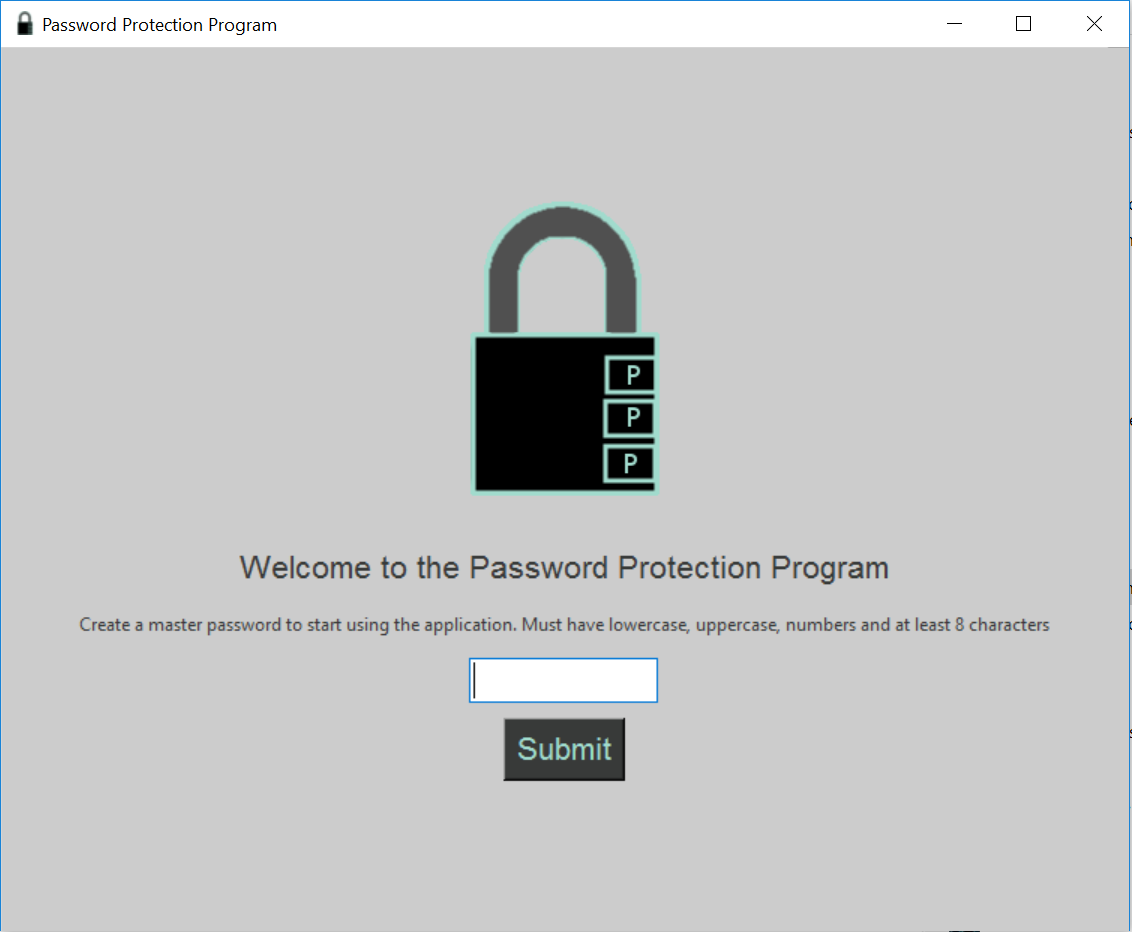
\includegraphics[scale=1.0]{images/CreateMasPass.PNG}
	\caption{Create Master Password Screen}
	\label{fig:crMasPass}
\end{figure}

\newpage
For all subsequent use of the product, the initial entry screen will only require entry of the aster password as shown in the following image.

\begin{figure}[h]
	\centering
	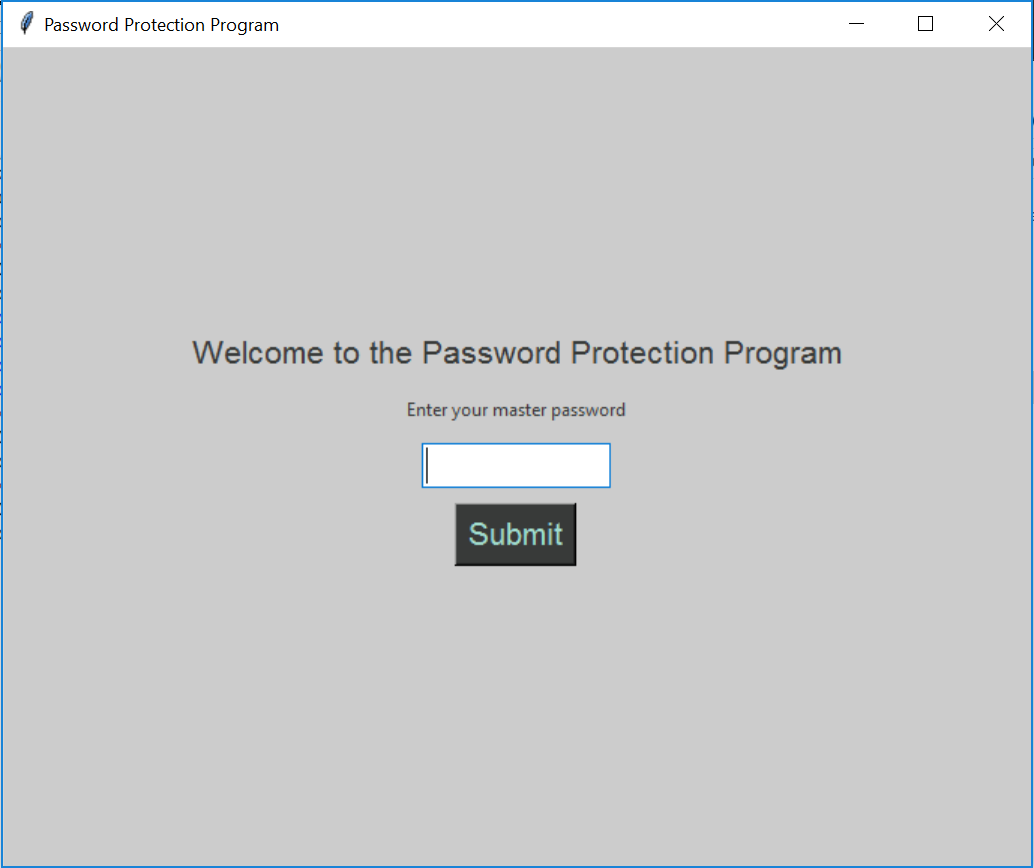
\includegraphics[scale=0.9]{images/EnterMasPass.PNG}
	\caption{Enter Master Password Screen}
	\label{fig:enMasPass}
\end{figure}


\newpage 
\subsection{System Menu} \label{SysMenu}

After creating a master password or logging into the system, the user is lead to a screen that in the center displays a brief description of the application. In the top left corner, the user is able to add new account usernames and passwords to the password manager by specifying the account name, type, username and password. Below this, starting with the master password, all the accounts for which the user has already saved a username and password are listed. 


\begin{figure}[h]
	\centering
	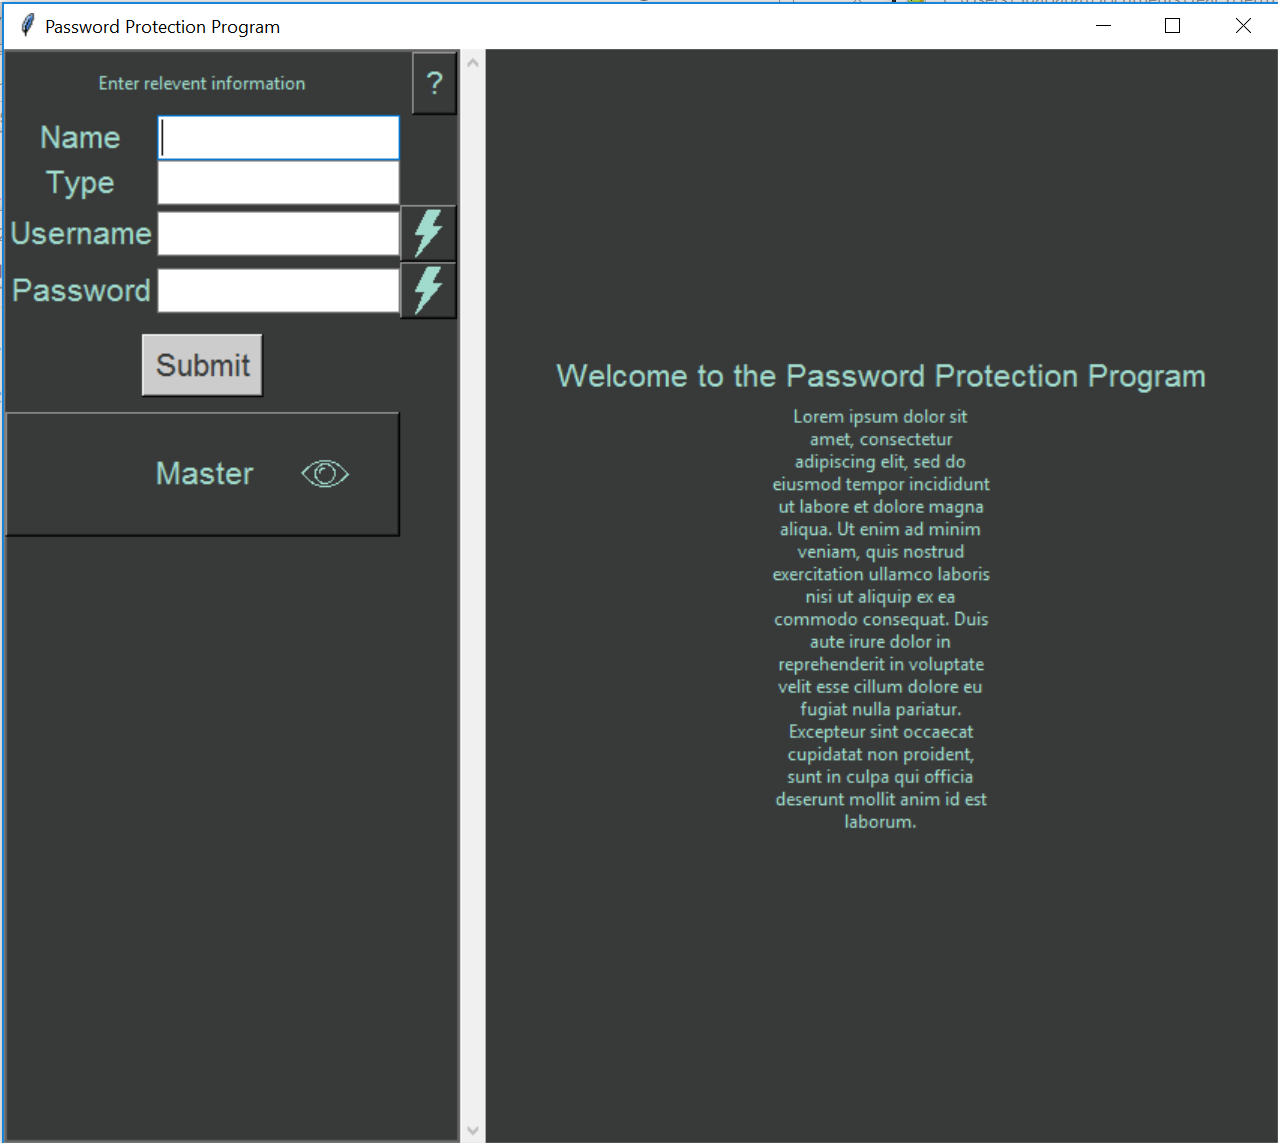
\includegraphics[scale=1.0]{images/InAppScreen.PNG}
	\caption{In Application Screen}
	\label{fig:InApp}
\end{figure}

\newpage
\subsection{Changing Master Password} \label{ChangeMasPass}

If the master password that was initially set for the software needs to be changed, this can be done so by choosing the master password box on the left side of the in-application screen.

\begin{figure}[h]
	\centering
	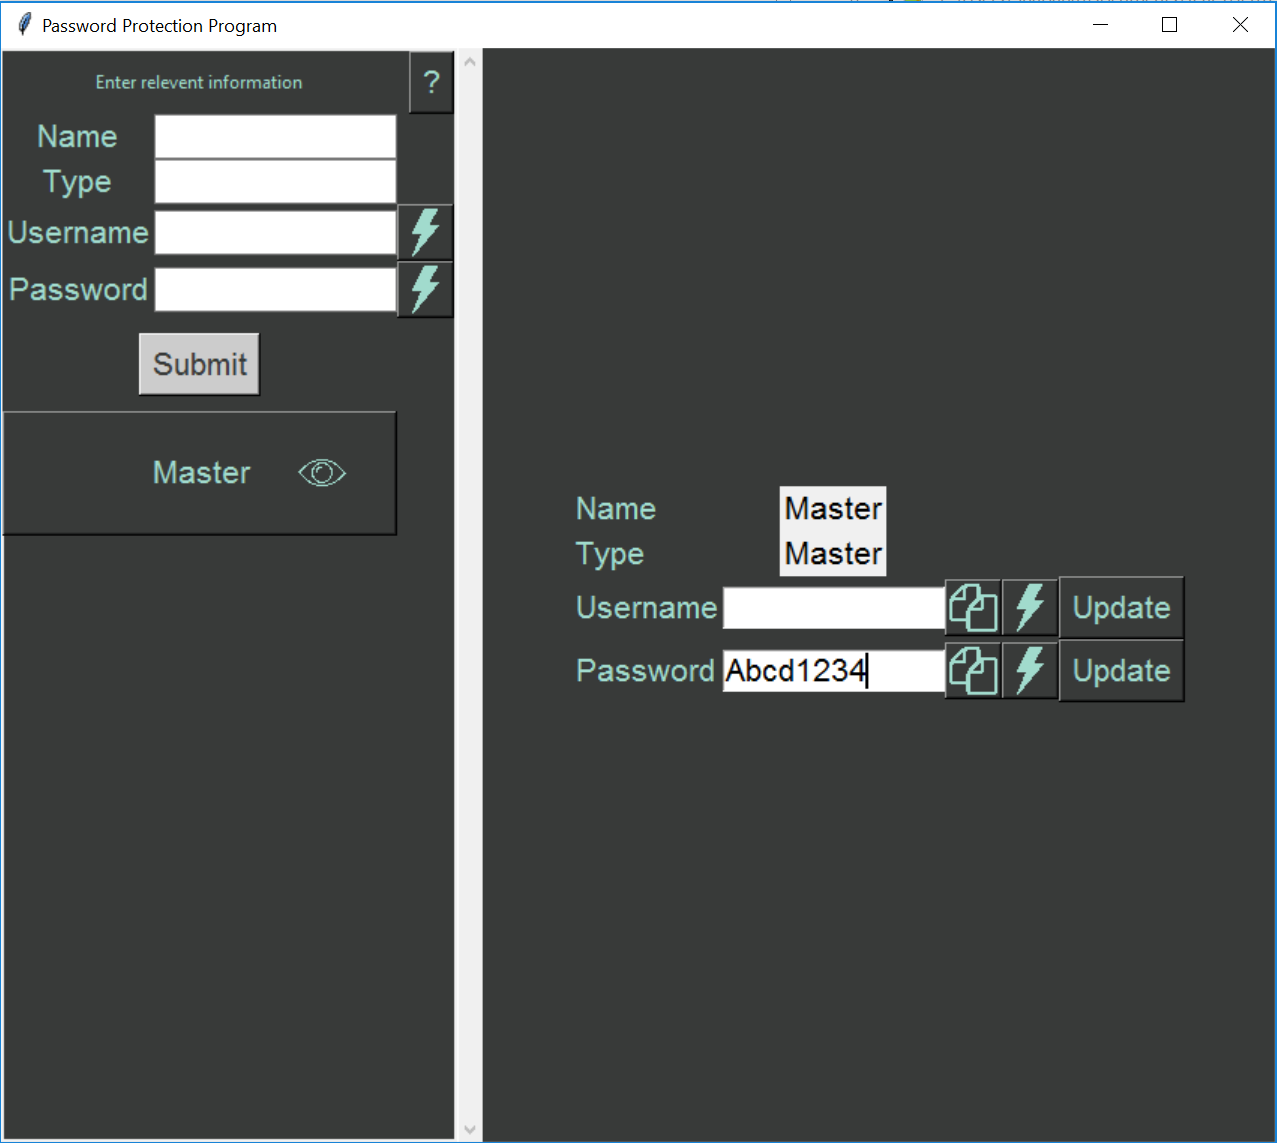
\includegraphics[scale=1.0]{images/ChangeMasPass.PNG}
	\caption{Changing Master Password}
	\label{fig:chMasPass}
\end{figure}


\subsection{Exit System} \label{SysExit}

The system can be exited by simply closing the application window as this automatically logs the user out as well. The application will also close after TIME AMOUNT of inactivity in order to preserve the security of the data.


\newpage
\section{Using the System} \label{SysUse}


\subsection{System Functions} \label{SysFunc}

\subsubsection{Add Entry} \label{AddEnt}

An account entry can be added to this password manager by filling out the required entry fields specified in the top left corner of the \hyperref[fig:InApp]{in-application screen}. The name of the entry will be used as a unique identifier for this entry account's information, the type is used for organization purposes and the username and password are those that the user has already associated with the specific account.

\begin{figure}[h]
	\centering
	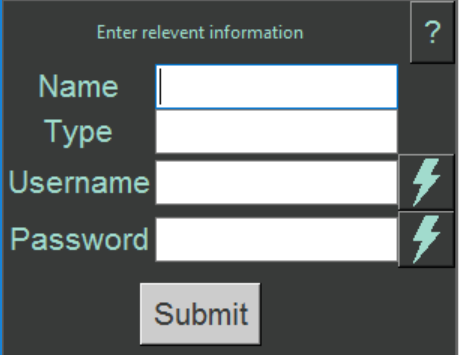
\includegraphics[scale=1.0]{images/AddEntry.PNG}
	\caption{Adding an Entry}
	\label{fig:AdEnt}
\end{figure}

\subsubsection{View Entry} \label{ViewEnt}

Once an entry has been added, it will be listed for viewing as a button in the menu on the left of the in-application screen. The entries are ordered from least recent to most recent entry, starting with the master password. The entry name is displayed on the button along with an eye sympbol to indicate the account that it is associated with.

\begin{figure}[h]
	\centering
	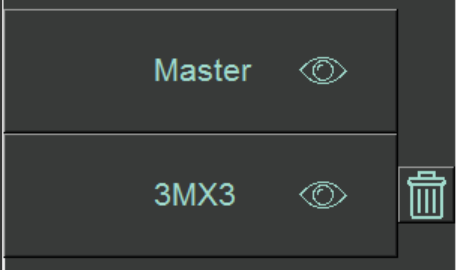
\includegraphics[scale=1.0]{images/ViewEntry.PNG}
	\caption{Button to View an Entry}
	\label{fig:VieEnt1}
\end{figure}

\newpage
After the button is clicked, all of the account information will be displayed in the center panel of the screen along with buttons for additional functions such as Copy, Generate and Update. 

\begin{figure}[h]
	\centering
	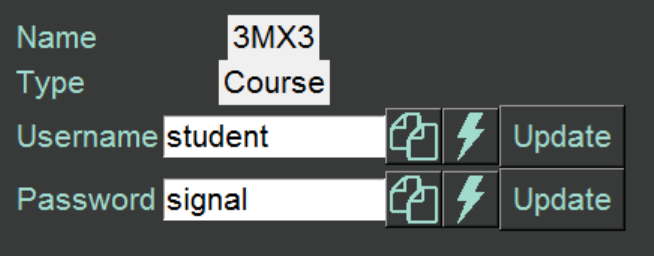
\includegraphics[scale=1.0]{images/UpdateEntry.PNG}
	\caption{Viewing an Entry}
	\label{fig:VieEnt2}
\end{figure}


\subsubsection{Delete Entry} \label{DelEnt}

An entry can be deleted at any time using the delete button located beside each account lising in the menu on the left of the screen. Obviously, the master password can not be deleted.

\begin{figure}[h]
	\centering
	
\includegraphics[scale=1.0]{images/DeleteEntry.PNG}
	\caption{Deleting an Entry}
	\label{fig:DeEnt}
\end{figure}

\subsubsection{Update Entry} \label{UpdateEnt}

An entry can be modified after it is selected in the menu and the information is displayed on the screen. Only the username and password for the selected account can be modified, if the user wishes to change the name and type of the account, the account must be deleted and recreated. After the desired fields are altered, to save these changes, the user must press the Update button located beside each field.

\begin{figure}[h]
	\centering
	
\includegraphics[scale=1.0]{images/Update.PNG}
	\caption{Updating an Entry}
	\label{fig:UpEnt}
\end{figure}

\subsubsection{Copy Field} \label{CopyField}

The copy button located beside the username and password fields is used to facilitate entering authentication information into the service the user wishes to use. The decrypted passoword or username is copied directly to keyboard when the corresponding copy button is pressed.

\begin{figure}[h]
	\centering
	
\includegraphics[scale=1.0]{images/Copy.PNG}
	\caption{Copying a Field}
	\label{fig:CopF}
\end{figure}

\subsubsection{Generate Field} \label{GenField}

The generate button, denoted by a lightning bolt, provides the user with a random, cryptographicaly sage 8 charater string consisting of upper and lower case alphabets and numbers. The user can use this generated value for their account if they wish.

\begin{figure}[h]
	\centering
	
\includegraphics[scale=1.0]{images/Generate.PNG}
	\caption{Generating a Username or Password}
	\label{fig:genPass}
\end{figure}

\subsubsection{User Manual} \label{UseMan}

If at any time the user is unsure of the function of a button, a user manual will be linked to the question mark button located on the top left corner of the in-application screen beside the add a new entry section.

\begin{figure}[h]
	\centering
	
\includegraphics[scale=1.0]{images/UserManual.PNG}
	\caption{Accessing the User Manual}
	\label{fig:UsMan}
\end{figure}

\subsection{Inactivity Timeout} \label{InacTime}

As PasswordProtectionProgram is a password manager, the primary concern of the application is the security of the user information. Therefore, the system is equipped with an automatic logout function when 2 minutes of inactivity is detected. In this way, the application is not left open when the user is not present and this prevents individuals other than the user from accessing the information.

\subsection{Special Instructions for Error Correction} \label{ErrCorr}

TENTATIVE: In the case that the master password is forgotten, the system has a "forgot master password" button that when pressed will reset the application to the state it was when first downloaded. Thus, all saved data will be lost and a new master password will have to be created.

%\section*{References}
\newpage

\bibliography{User}
\bibliographystyle{ieeetr}



\end{document}
